%-*-coding: utf-8-*-
\chapter{Теоретическое решение}

\section{Предобработка данных}

Для решения поставленной задачи первым делом необходимо построить
навигационный граф. Подразумевается, что карта содержит множество
контуров, которые можно классифицировать на ограничивающие воду и
ограничивающие сушу. Контура заданы как последовательности точек в
плоской проекции Меркатора~\cite{thomas1952conformal}. Для построения
графа выполняется определённый набор действий.

Первым делом происходит упрощение водных контуров, полученных из карты, и
объединение их в один полигон. Упрощение выполняется по двум причинам:
\begin{itemize}
    \item Хоть такая модификация и может повлиять на корректность
      маршрута, действительно сильно некорректных маршрутов от неё
      появиться не может. Неформальная постановка задачи допускает
      такие модификации. Кроме того, планируется искать маршруты по
      всему земному шару, поэтому мелкомасштабные детали не несут
      никакой информации.
    \item Данные с мелкомасштабной морской карты содержат слишком
      много точек, из-за чего в навигационном графе будет крайне много
      вершин и рёбер, если не упрощать контура. Это приведёт к тому,
      что граф будет занимать слишком много памяти, а поиск путей в
      нём будет занимать слишком много времени.
\end{itemize}
Для упрощения используется алгоритм Дугласа-Пекера~\cite{douglas1973algorithms}.

После построения единого полигона, описывающего контуры воды, для него
строится straight~skeleton~\cite{aichholzer1996straight}, с помощью
которого выполняется смещение полигона внутрь. Это делается по
следующим причинам:
\begin{itemize}
    \item Корабли не плавают слишком близко к суше. При этом стоит в
      очередной раз отметить, что в данной задаче не требуется искать
      кратчайший маршрут, а требуется получать естественные маршруты,
      которые потенциально могут использоваться для реальных кораблей.
    \item Маршруты, проходящие по границе суши, хуже визуализируются,
      поскольку перемешиваются с сушей. В то же время при визуализации
      маршрутов, проходящих на небольшом расстоянии от суши, таких
      проблем не возникает.
    \item Такая модификация позволяет нейтрализует возможные нарушения
      корректности маршрута, возникающие из-за упрощения контуров.
      Если при упрощении любая точка смещается на расстояние не больше
      $l$, а смещение контура происходит на расстояние $d > l$, то про
      любую точку, принадлежащую итоговому полигону, можно сказать,
      что в исходной карте она точно принадлежит контуру с водой.
\end{itemize}

По смещённому полигону строится навигационный граф. Для этого на
плоскости, на которую спроецирована карта, строится сетка с некоторым
постоянным шагом. Для каждого ребра сетки проверяется принадлежность
полигону, ограничивающему воду. Если ребро полностью принадлежит
полигону, то оно добавляется в граф (вместе с инцидентным вершинами).
Помимо этого в граф добавляются все вершины полигона и рёбра до
видимых вершин (то есть рёбра, полностью принадлежащие полигону) в
некотором радиусе. При этом важно ограничить максимальную длину ребра.
Это связано с тем, что граф строится по полигону в плоской проекции,
проверка принадлежности отрезка полигону также выполняется в плоской
проекции. В то же время кратчайшее расстояние между двумя точками на
Земле достигается не для отрезка, а для дуги (приближённо). Поэтому
такая проверка, вообще говоря, некорректна. Однако, если ограничить
длину ребра, то отклонение дуги от отрезка будет невелико. Учитывая
то, что полигон смещён внутрь, можно утверждать, что любое ребро
действительно будет проходить по воде, не пересекая препятствия.

Также в полученный граф добавляются дополнительные рёбра. Во-первых,
добавляются рёбра, получившиеся в результате «схлопывания» контуров
полигона при построении straight skeleton'а. При этом они также
упрощаются. Это необходимо сделать, потому что при смещении полигона
некоторые контура «схлопываются», объединяясь в один. Если между ними
был, скажем, какой-нибудь канал, то по нему нельзя будет пройти в
итоговом графе. Именно поэтому такие рёбра из straight skeleton'а
добавляются в граф. Во-вторых, поскольку граф строится по контурам в
проекции Меркатора, то в нём отсутствуют рёбра через 180-ый меридиан.
Такие рёбра также добавляются в граф.

\FloatBarrier

\section{Поиск одного маршрута}

Прежде чем перейти к описанию алгоритма поиска семейств маршрутов,
необходимо детально описать процесс поиска одного маршрута в
построенном навигационном графе. Первым делом для двух заданных точек
проверяется принадлежность полигону, ограничивающему воду. Если точки
действительно находятся на воде, то по имеющейся сетке для них
находятся ближайшие вершины графа, и все корректные рёбра до ближайших
вершин добавляются в граф. После этого используется алгоритм
Дейкстры~{dijkstra1959note} для поиска кратчайшего пути в графе между
этими двумя вершинами. Поиск останавливается, когда кратчайший путь до
нужной вершины найден. Поскольку найденный путь не является
действительно кратчайшим маршрутом между двумя точками, производится
попытка его сократить. Для каждой вершины пути проверяется, можно ли
её убрать из маршрута, не нарушив его корректность и не увеличив длину
пути. Если можно, то такая вершина убирается из маршрута. Этот процесс
может повторяться несколько раз, для чего каждый отрезок пути
разбивается на подотрезки меньшей длины. После этого опять
производится попытка выкинуть точки. И так далее. Ещё одна модификация
вызвана тем, что в связи со структурой графа в маршруте могут
появляться слишком острые углы (если в каком-нибудь контуре,
образованном при смещении полигона, есть острый угол). В реальных
маршрутах не бывает острых углов, поэтому выполняется сглаживание
маршрута, то есть замена острого угла ломаной, аппроксимирующей дугу
эллипса. При этом корректность такой замены проверяется по исходному
полигону, не смещённому внутрь.

\begin{figure}
    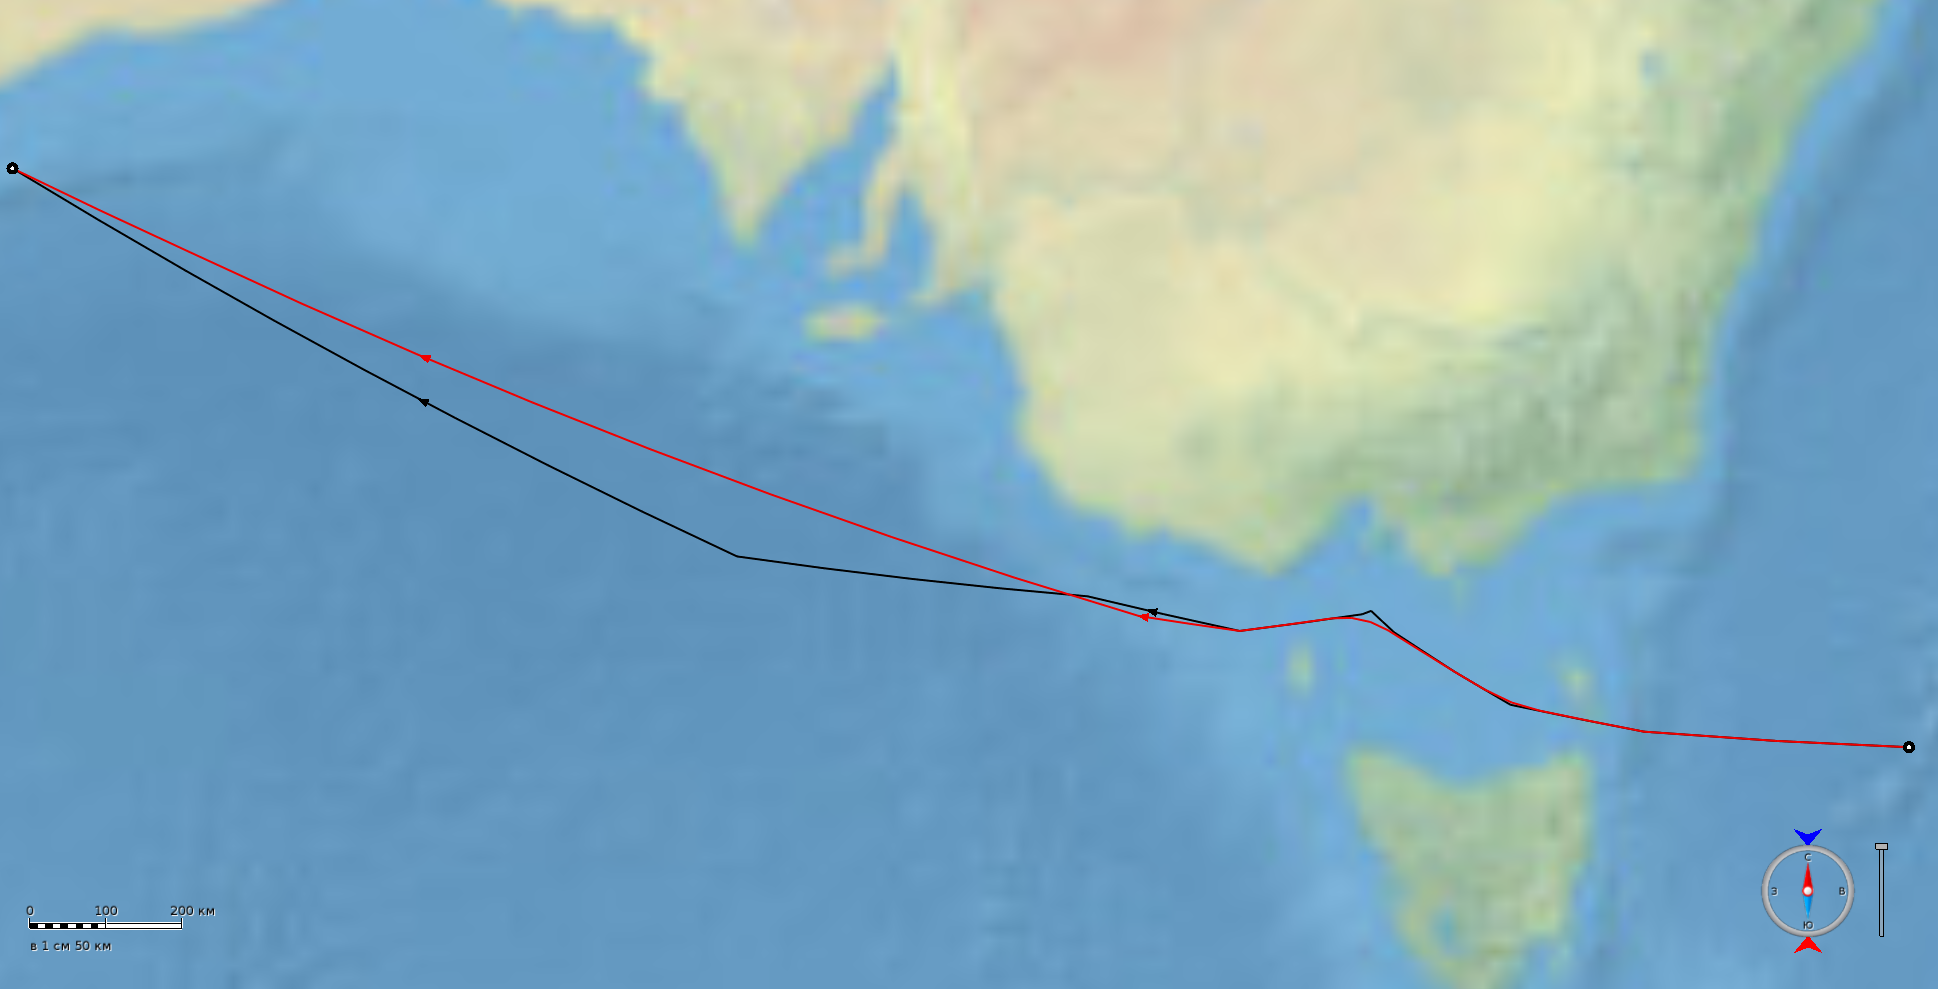
\includegraphics[width=\textwidth]{Solution/shortcut-and-smoothing}
    \caption{Сокращение и сглаживание маршрута}
    \label{fig:path-improvements}
\end{figure}

На рисунке \ref{fig:path-improvements} продемонстрирован эффект от
сокращения и сглаживания маршрута. Чёрной линией изображён кратчайший
путь в графе, а красной --- итоговый маршрут. Нетрудно видеть, что
левая часть маршрута сократилась, а в правой части произошло
сглаживание, что сделало маршрут более естественным.

\FloatBarrier

\section{Поиск нескольких маршрутов}

\FloatBarrier

